\section{MCP server(serena) 설치}

\subsection{uv 설치}
UV는 Rust로 만들어진 Python 패키지 관리자로, pip보다 10-100배 빠른 속도로 패키지를 설치합니다. Serena MCP Server는 여러 Python 패키지가 필요한데, UV를 사용하면 이런 패키지들을 빠르게 설치할 수 있습니다. 또한 프로젝트마다 독립된 환경을 만들어 패키지 간 충돌을 방지합니다.
\begin{figure}[H]
    \centering
    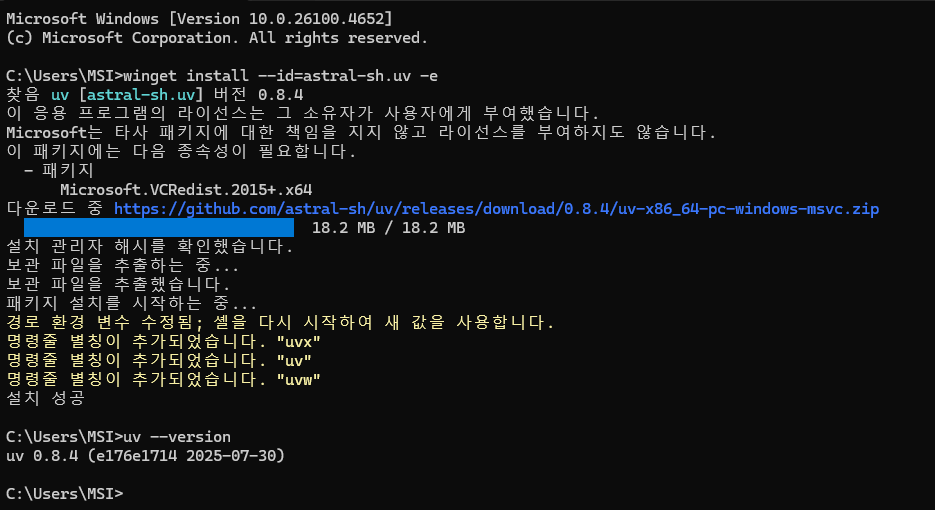
\includegraphics[width=0.5\textwidth]{1/image11.png}
    \caption{uv 설치}
    \label{fig:uv_install}
\end{figure}
UV의 가장 큰 장점은 통합성과 속도인데, Python 설치부터 패키지 관리까지 한 번에 처리하며, 병렬 처리와 캐싱 기능으로 반복 작업 시 시간을 크게 단축시킵니다. 기존 pip 명령어와 requirements.txt를 그대로 사용할 수 있어 추가 학습 없이 바로 활용 가능합니다. 결과적으로 MCP Server 설치 시간이 대폭 감소하고, 프로젝트 간 패키지 버전 충돌 문제가 해결됩니다. 이를 통해 환경 설정에 소요되는 시간을 줄이고 실제 개발 작업에 집중할 수 있습니다.

\subsection{serena MCP 설치}
Serena MCP Server를 설치하기 위해 Git을 사용하여 소스 코드를 다운로드합니다.
\begin{figure}[H]
    \centering
    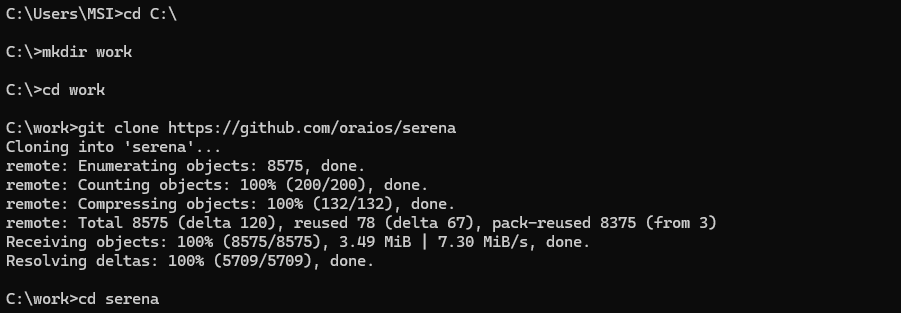
\includegraphics[width=0.5\textwidth]{1/image12.png}
    \caption{serena 설치}
    \label{fig:serena_install}
\end{figure}\textbackslash{
{git clone \href{https://github.com/erelon/serena\%7D}{https://github.com/erelon/serena\}} 명령어로 GitHub에 있는 Serena 저장소의 전체 코드를 로컬 컴퓨터로 복사합니다. Git은 버전 관리 시스템으로, \{clone\} 명령어는 원격 저장소의 모든 파일, 폴더, 그리고 변경 이력까지 함께 가져옵니다.
실행 과정을 보면 Git이 먼저 원격 저장소의 객체들을 확인하고(Enumerating), 개수를 세고(Counting), 압축하여(Compressing) 전송합니다. 총 8575개의 객체 중 3375개는 델타 압축을 통해 효율적으로 전송되며, 최종적으로 7.39 MiB의 데이터를 받습니다.
클론이 완료되면 현재 디렉토리에 'serena'라는 새 폴더가 생성됩니다. \{cd serena\} 명령어로 이 폴더로 이동하면, Serena MCP Server의 모든 소스 코드와 설정 파일을 확인할 수 있습니다. 이제 UV를 사용하여 필요한 Python 패키지들을 설치하고 서버를 실행할 준비가 완료됩니다.

\subsection{Claude code와 통합}
글자